\documentclass[11pt,a4paper]{article}
\usepackage[latin1]{inputenc}
\usepackage{framed}

\setlength{\parindent}{0pt}
\setlength{\parskip}{3ex}

% My settings
\usepackage{algorithm, algorithmic, listings} % Code
\usepackage{amsmath,amstext,amssymb,amsfonts,cancel,dsfont,mathtools} % Math
\usepackage{color, xcolor} % Color
\usepackage{diagbox, tabularx} % Table
\usepackage{enumerate} % List
\usepackage{epsfig, epstopdf, graphicx, multicol, multirow, palatino, pgfplots, subcaption, tikz} % Image
\usepackage{fancybox}
\usepackage{verbatim}

\usepackage[font=footnotesize]{caption} % labelfont=bf
\usepackage[font=scriptsize]{subcaption} % labelfont=bf
\usepackage[margin=1in]{geometry}
\usepackage[hidelinks]{hyperref}
\epstopdfsetup{outdir=./Figure/Converted/}
\graphicspath{{./Figure/}}

\makeatletter
\def\input@path{{./Figure/}}
\makeatother

\pgfplotsset{compat=1.13}

\lstset{
basicstyle=\footnotesize,
breaklines=true,
frame=tb,
tabsize=2,
showstringspaces=false,
numbers=left,
showtabs=false,
commentstyle=\color{green},
keywordstyle=\color{blue},
stringstyle=\color{red},
emph={then},
emphstyle=\color{blue}
}

\begin{document}
\title{\sc\vspace{3cm}\hrule\vspace{0.3cm}{\LARGE DD2380}\\\vspace{0.1cm}{\Large Artificial Intelligence}\vspace{0.3cm}\hrule\vspace{1.5cm}{\Large Assignment 3}\\{\large Knowledge, Reasoning, and Planning}}
\author{Jiang, Sifan\\sifanj@kth.se}
\maketitle
\newpage


\section{Maze Runner}


\section{Student Einstein Puzzle}
\subsection{E-level 10 points}
\begin{itemize}
	\item S1: $Commute(John) = Bike$
	\item S2: $Commute(Carol) = Bike$
	\item S3: $Company(Carol) = W$
	\item S4: $Commute(Mary) = Subway$
	\item S5: $Coworkers(Mary, Carol)$
	\item S6: $\lnot Classmates(Mary, Carol)$
	\item S7: $\forall x. \; Commute(x) = Bike \implies University(x) = KTH$
	\item S8: $\forall x. \; University(x) = KTH \implies Classmates(Sofie, x)$
	\item S9: $\forall x. \; Classmates(Carol, x) \wedge \lnot x = Carol \implies Comany(x) = Z$
	\item S10: $\forall x. \; Commute(x) = Subway \wedge Company(x) = W \implies University(x) = SU$
	\item S11: $\forall x. \; Coworkers(John, x) \implies Commute(x) = Walk$
\end{itemize}

\subsection{E-level 5 points}
\par Let $\theta = \left\{ x / John \right\}$, and first take premises S1 and S7 into consideration. We would have
$$
\frac{X1: Commute(John) = Bike, \; X2: Commute(x) = Bike \implies University(x) = KTH}{X3: University(John) = KTH},
$$
where $\theta = \left\{ x / John \right\}$. Let \textbf{T1}: $University(John) = KTH$.

\par Then take T1 and S7 into consideration. We would have
$$
\frac{X1: University(John) = KTH, \; X2: University(x) = KTH \implies Classmates(Sofie, x)}{X3: Classmates(Sofie, John)},
$$
where $\theta = \left\{ x / John \right\}$.  Thus, $Classmates(Sofie, John)$ is inferred.

\subsection{D-level 10 points}
\begin{itemize}
	\item C1: $Commute(John) = Bike$
	\item C2: $Commute(Carol) = Bike$
	\item C3: $Company(Carol) = W$
	\item C4: $Commute(Mary) = Subway$
	\item C5: $Coworkers(Mary, Carol)$
	\item C6: $\lnot Classmates(Mary, Carol)$
	\item C7: $\lnot Commute(x) = Bike \vee University(x) = KTH$
	\item C8: $\lnot University(x) = KTH \vee Classmates(Sofie, x)$
	\item C9: $\lnot Classmates(Carol, x) \vee x = Carol \vee Comany(x) = Z$
	\item C10: $\lnot Commute(x) = Subway \vee \lnot Company(x) = W \vee University(x) = SU$
	\item C11: $\lnot Coworkers(John, x) \vee Commute(x) = Walk$
\end{itemize}

\subsection{C-level 15 points}
\begin{itemize}
	\item C12: If two students are co-workers, then they work at the same company.
	\item C13: If two students work at the same company, then they are co-workers.
	\item C14: If this student is the co-worker of that student, then that student is also the co-worker of this student.
	\item C15: If this student is the classmate of that student, then that student is also the classmate of this student.
	\item C16: If two students are classmates, then they study at the same university.
	\item C17: If two students study at the same university, then they are classmates.
\end{itemize}

\par To infer the information of each students:
\begin{itemize}
	\item From C1, C2, C3, and C4, we can get
	\begin{align*}
		& Commute(John) = Bike \\
		& Commute(Carol) = Bike \\
		& Company(Carol) = W \\
		& Commute(Mary) = Subway
	\end{align*}
	
	\item From C1 and C7, we can have $l_{1}$ is $Commute(John) = Bike$, $m_{1}$ is $\lnot Commute(x) = Bike$, $m_{2}$ is $University(x) = KTH$, and $UNIFY(l_{1}, \lnot m_{1}) = \theta = \left\{ x/John \right\}$. The resolvent clause is $University(John) = KTH$. The resolution is
	$$
	\frac{X1: Commute(John) = Bike, X2: \lnot Commute(x) = Bike \vee University(x) = KTH}{X3: University(John) = KTH},
	$$
	where $\theta = \left\{ x/John \right\}$. Let \textbf{A1}: $University(John) = KTH$.
	
	\item From C2 and C7, we can have $l_{1}$ is $Commute(Carol) = Bike$, $m_{1}$ is $\lnot Commute(x) = Bike$, $m_{2}$ is $University(x) = KTH$, and $UNIFY(l_{1}, \lnot m_{1}) = \theta = \left\{ x/Carol \right\}$. The resolvent clause is $University(Carol) = KTH$. The resolution is
	$$
	\frac{X1: Commute(Carol) = Bike, X2: \lnot Commute(x) = Bike \vee University(x) = KTH}{X3: University(Carol) = KTH},
	$$
	where $\theta = \left\{ x/Carol \right\}$. Let \textbf{A2}: $University(Carol) = KTH$.
	
	\item From A1 and C8, we can have $l_{1}$ is $University(John) = KTH$, $m_{1}$ is $\lnot University(x) = KTH$, $m_{2}$ is $Classmates(Sofie, x)$, and $UNIFY(l_{1}, \lnot m_{1}) = \theta = \left\{ x/John \right\}$. The resolvent clause is $Classmates(Sofie, John)$. The resolution is
	$$
	\frac{X1: University(John) = KTH, X2: \lnot University(x) = KTH \vee Classmates(Sofie, x)}{X3: Classmates(Sofie, John)},
	$$
	where $\theta = \left\{ x/John \right\}$. Let \textbf{A3}: $Classmates(Sofie, John)$.
	
	\item From A1 and C15, we can have the resolution
	$$
	\frac{X1: Classmates(Sofie, John), X2: \lnot Classmates(x, y) \vee Classmates(y, x)}{X3: Classmates(John, Sofie)},
	$$
	where $\theta = \left\{ x/Sofie, \; y/John \right\}$. Let \textbf{A4}: $Classmates(John, Sofie)$.
	
	\item From A1, A4, and C16, we can have the resolution
	$$
	\frac{X1: A1, X2: A4, X3: \lnot Classmates(x, y) \vee \lnot University(x) = z \vee University(y) = z}{X4: University(Sofie) = KTH},
	$$
	where $\theta = \left\{ x/John,\; y/Sofie,\; z/KTH \right\}$. Let \textbf{A5}: $University(Sofie) = KTH$.
	
	\item From A1, A2 and C17, we can have the resolution
	$$
	\frac{X1: A1, X2: A2, X3: Classmates(x, y) \vee \lnot University(x) = z \vee \lnot University(y) = z}{X4: Classmates(Carol, John)},
	$$
	where $\theta = \left\{ x/Carol,\; y/John,\; z/KTH \right\}$. Let \textbf{A6}: $Classmates(Carol, John)$.
	
	\item From A2, A5, and C17, we can have \textbf{A7}: $Classmates(Carol, Sofie)$, which is similar to how we get A6.
	
	\item From A6, C9, and C19, we can have $l_{1}$ is $Classmates(Carol, John)$, $l_{2}$ is $\lnot Carol = John$, $m_{1}$ is $\lnot Classmates(Carol, x)$, $m_{2}$ is $x = Carol$, $m_{3}$ is $Company(x) = Z$, and $UNIFY(l_{1}, \lnot m_{1}) = \theta = \left\{ x/John \right\}$. The resolvent clause is $Company(John) = Z$. The resolution is
	$$
	\frac{X1: A1, X2: C19, X3: \lnot Classmates(Carol, x) \vee x = Carol \vee Comany(x) = Z}{X4: Company(John) = Z},
	$$
	where $\theta = \left\{ x/John \right\}$. Let \textbf{A8}: $Company(John) = Z$.
	
	\item From A7, C9, and C21, we can have \textbf{A9}: $Company(Sofie) = Z$, which is similar to how we get A8.
	
	\item From A8, A9, and C13, we can have the resolution
	$$
	\frac{X1: A8, X2: A9, X3: \lnot Company(x) = z \vee \lnot Company(y) = z \vee Coworkers(x, y)}{X4: Coworkers(John, Sofie)},
	$$
	where $\theta = \left\{ x/John, y/Sofie, z/Z \right\}$. Let \textbf{A10}: $Coworkers(John, Sofie)$.
	
	\item A10 and C11, we can have $l_{1}$ is $Coworkers(John, Sofie)$, $m_{1}$ is $\lnot Coworkers(John, x)$, $m_{2}$ is $Commute(x) = Walk$, and $UNIFY(l_{1}, \lnot m_{1}) = \theta = \left\{ x/Sofie  \right\}$. The resolvent clause is $Commute(Sofie) = Walk$. The resolution is
	$$
	\frac{X1: Coworkers(John, Sofie), X2: \lnot Coworkers(John, x) \vee Commute(x) = Walk}{X3: Commute(Sofie) = Walk},
	$$
	where $\theta = \left\{ x/Sofie \right\}$. Let \textbf{A11}: $Commute(Sofie) = Walk$.
	
	\item From C5 and C14, we can have \textbf{A12}: $Coworkers(Carol, Marry)$, which is similar to how we get A4.
		
	\item From A12, C3, and C12, we can have the resolution
	$$
	\frac{X1: A12, X2: C3, X3: \lnot Coworkers(x, y) \vee \lnot Company(x) = z \vee Company(y) = z}{X4: Company(Marry) = W},
	$$
	where $\theta = \left\{ x/Carol, y/Marry, z/W \right\}$. Let \textbf{A13}: $Company(Marry) = W$.
	
	\item From A13, C4, and C10, we can have the resolution
	$$
	\frac{X1: Commute(Marry) = Subway, X2: Company(Marry) = W, X3: C10}{X4: University(Marry) = SU}
	$$
	where $\theta = \left\{ x/Marry \right\}$. Let \textbf{A14}: $University(Marry) = SU$.
\end{itemize}

\par In all, we would get
\begin{table}[!ht]
	\caption{The information of each students.}
	\label{tab:2.4}
	\centering
	\begin{tabular}{|l|l|l|l|}
	\hline
	Name 	& Commute 	& Company 	& University 	\\\hline\hline
	Carol 	& Bike		& W			& KTH			\\\hline
	John 	& Bike 		& Z 		& KTH 			\\\hline
	Mary 	& Subway 	& W 		& SU			\\\hline
	Sofie 	& Walk 		& Z 		& KTH 			\\\hline	
	\end{tabular}
\end{table}

\subsection{C-level 5 points}
\par Assume we have two grounded clauses: $A \wedge \lnot B$, $\lnot A \wedge B$. What we can get are $A \wedge \lnot A$ and $B \wedge \lnot B$.


\section{Florence + The Machine at Ericsson Globe}
\subsection{E-level 10 points}
\label{3-1}
\par A part of the reachable space of all states containing 10 different states is illustrated in fig~\ref{fig:3-1}.
\begin{figure}[!htbp]
	\footnotesize
	\centering
	\includegraphics[width=\textwidth]{3-1}
	\caption{A part of the reachable space of all states.}
	\label{fig:3-1}
\end{figure}

\subsection{E-level 5 points}
\begin{itemize}
	\item Infinity. One can keep travelling between two stations by taking actions $GoForth(x, y)$ and $GoBack(y, x)$, where $x$ and $y$ are two different stations.
	\item Infinity. The reason is same with above question even though $Travel(Gp, Gp, GB)$ is removed.
	\item 12 actions: $GetOnBus(RB, Th)$ $\rightarrow$ $GoForth(Th, Sl)$ $\rightarrow$ $GoForth(Sl, Mt)$ $\rightarrow$ \\ $GetOffBus(RB, Mt)$ $\rightarrow$ $PickTicket(Mt)$ $\rightarrow$ $GetOnBus(RB, Mt)$ $\rightarrow$ $GoBack(Mt, Sl)$ $\rightarrow$ $GetOffBus(RB, Sl)$ $\rightarrow$ $GetOnBus(GB, Sl)$ $\rightarrow$ $GoForth(Sl, Gp)$ $\rightarrow$ $GoForth(Gp, Gl)$ $\rightarrow$ $GetOffBus(GB, Gl)$.
\end{itemize}

\subsection{E-level 10 points}
\label{3-3}
\par The space of all belief states that are reachable from the initial one is illustrated in fig~\ref{fig:3-3}.
\begin{figure}[!htbp]
	\footnotesize
	\centering
	\includegraphics[width=\textwidth]{3-3}
	\caption{The space of all belief states that are reachable from the initial one.}
	\label{fig:3-3}
\end{figure}

\begin{itemize}
	\item Always true:
		\begin{enumerate}[(1)]
			\item $Travel(Th, Sl, RB)$;
			\item $Travel(Sl, Mt, RB)$;
			\item $Travel(Sl, Gp, GB)$.
		\end{enumerate}			
		\par Always false:
		\begin{enumerate}[(1)]
			\item $BusAt(RB, Gp)$;
			\item $BusAt(RB, Gl)$;
			\item $BusAt(GB, Th)$.
		\end{enumerate}
	\item $5$ actual physical states. We don't know whether we are at $Th$, $Sl$, $Mt$, $Gp$, or $Gl$, but we know we are not at on the bus, so the initial belief state contains $5$ actual physical states which is illustrated in fig~\ref{fig:3-3}.
	\item $0$. There's no feasible actions can be applied to the initial belief state, not to say finding the plans that lead to the satisfaction of the goal.
	\item There is no plan that lead to the satisfaction of the goal.
\end{itemize}

\subsection{D-level 10 points}
\par A part of the reachable belief state space containing $5$ states with their outgoing edges labelled with ground actions is illustrated in fig~\ref{fig:3-4}.
\begin{figure}[!htbp]
	\footnotesize
	\centering
	\includegraphics[width=\textwidth]{3-4}
	\caption{A part of the reachable belief state space.}
	\label{fig:3-4}
\end{figure}

\begin{itemize}
	\item $64$ actual physical states. We cannot observe whether we are on a bus, and whether we have a ticket, so $YouOnBus$ and $YouHaveTicket$ are unknown. Also, although we know we are at $Th$, we still don't know whether we are at $Sl$, $Mt$, $Gp$, and $Gl$ or not. In all we have $6$ unknown fluents, meaning the initial belief state contains $2^{6} = 64$ actual physical states.
	\item Infinity. We can keep travelling between two stations, for example, by taking actions $GoToSl$ and $GoToTh$ after $YouOnBus$ becoming true.
	\item $7$ actions: $GetOnBus(Th)$ $\rightarrow$ $GoToMt$ $\rightarrow$ $GetOffBus(Mt)$ $\rightarrow$ $PickTicket(Mt)$ $\rightarrow$ \\ $GetOnBus(Mt)$ $\rightarrow$ $GoToGl$ $\rightarrow$ $GetOffBus(Gl)$.
\end{itemize}

\subsection{C-level 10 points}
\par A connected subgraph of the belief state space containing $10$ different belief states assuming that we initially do not know where our friend lives is illustrated in fig~\ref{fig:3-5}.
\begin{figure}[!htbp]
	\footnotesize
	\centering
	\includegraphics[width=\textwidth]{3-5}
	\caption{A connected subgraph of the belief state space containing $10$ different belief states assuming that we initially do not know where our friend lives.}
	\label{fig:3-5}
\end{figure}

\par One feasible contingent plan is illustrated in listing~\ref{list:3-5}.
\begin{lstlisting}[language=C++, caption={One feasible contingent plan.}, label=list:3-5]
if TicketAtFriend(Th)
then[PickTicket(Th), GetOnBus(RB,Th), GoForth(Th,Sl), GetOffBus(RB,Sl), GetOnBus(GB,Sl), GoForth(Sl,Gp), GoForth(Gp,Gl), GetOffBus(GB,Gl)]
else[GetOnBus(RB,Th), GoForth(Th,Sl), GetOffBus(RB,Sl), if TicketAtFriend(Sl)
	then[PickTicket(Sl), GetOnBus(GB,Sl), GoForth(Sl,Gp), GoForth(Gp,Gl), GetOffBus(GB,Gl)]
	else[GetOnBus(RB,Sl), GoForth(Sl,Mt), GetOffBus(RB,Mt), if TicketAtFriend(Mt)
		then[PickTicket(Mt), GetOnBus(RB,Mt), GoBack(Mt,Sl), GetOffBus(RB,Sl), GetOnBus(GB,Sl), GoForth](Sl,Gp), GoForth(Gp,Gl), GetOffBus(GB,Gl)]
		else[GetOnBus(RB,Mt), GoBack(Mt,Sl), GetOffBus(RB,Sl), GetOnBus(GB,Sl), GoForth](Sl,Gp), GetOffBus(GB,Gp), if TicketAtFriend(Gp)
			then[PickTicket(Gp), GetOnBus(GB,Gp), GoForth(Gp,Gl), GetOffBus(GB,Gl)]
			else[GetOnBus(GB,Gp), GoForth(Gp,Gl), GetOffBus(GB,Gl), if TicketAtFriend(Gl)
				then[PickTicket(Gl)]
				else[NoOp]
			]
		]
	]
]
\end{lstlisting}

\subsection{B-level 15 points}
\begin{itemize}
	\item The size of the state space in the first fully observable case can either be smaller or larger than the size of the belief state space in the second sensorless case.
	\begin{itemize}
		\item Fully observable case \textbf{smaller than} sensorless case: taking the example in fig~\ref{fig:3-6-1} as the example of the fully observable case.
		\begin{figure}[!htbp]
			\footnotesize
			\centering
			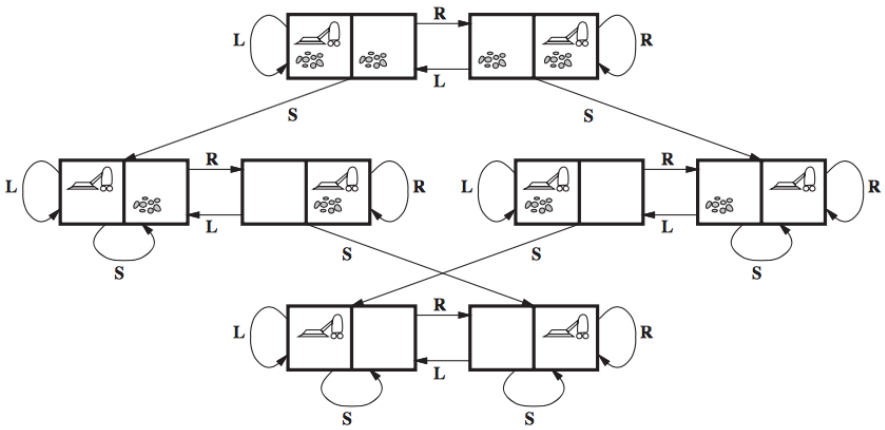
\includegraphics[width=.75\textwidth]{3-6-1}
			\caption{The fully observable case.}
			\label{fig:3-6-1}
		\end{figure}
		\par Assuming for the sensorless case, we don't know the position of the robot. Then the initial belief state would be the same with fig~\ref{fig:3-6-2}.
		\begin{figure}[!htbp]
			\footnotesize
			\centering
			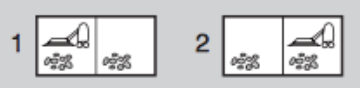
\includegraphics[scale=.5]{3-6-2}
			\caption{The initial belief state of sensorless case.}
			\label{fig:3-6-2}
		\end{figure}
		\par If we apply $L$ or $R$ to the initial belief state, we would get the one of the state on the top of the fully observable case, thus the size of the state space of the fully observable case would be smaller than the size of the belief state space of the sensorless case.
		
		\item Fully observable case \textbf{larger than} sensorless case: If there's no actions can be applied to the initial belief state, than the size of the belief state space in the second sensorless case would be $1$. Then the size of the state space in the first case would be larger than the size of the belief state space in the second case. For example, the case in \ref{3-1} is fully observable and the size of the state space is bigger than $1$, while the case in \ref{3-3} is sensorless and the size of the belief state space is $1$.
	\end{itemize}
	
	\item The size of the representation of the initial state in the first fully observable case is always larger than the size of the representation of the initial belief state in the second sensorless case.
	\par Assume the number of the fluent that are unfixed (meaning not always being true or false) is $N$. Then for the fully observable case, there would be $N$ fluents listed in the state, thus, the size of the representation of the initial state is $N$.
	\par For the sensorless case, assume we have $M$ fluents are unknown. Then we would also have $N-M$ fluents are known. If we are using the \textit{open-world assumption}, the size of the representation of the initial belief state for the sensorless case is $N-M$. Since $M>1$, the size of the representation of the initial state in the first fully observable case is always larger than the size of the representation of the initial belief state in the second sensorless case.
\end{itemize}


\section{Sweet Cup}
\subsection{C-level 10 points}
\begin{itemize}
	\item Compare the initial state with the the goal state and ignore all preconditions,  the $Sweet(Cup)$ can then be achieved by $Stir(Cup)$, so the value of $h_{1}$ for the initial state is $2$.
	\item Remove all negative literals from effects, the $HasSugar(Teaspoon)$ would always be true after $FillTeaspoon()$ no matter $PourSugar(Cup)$ is conducted or not, while at the same time $Empty(Teaspoon)$ is also always true. Also, $Dry(Teaspoon)$ is always true. So all the plans is illustrated in fig~\ref{fig:4-1}.
	\begin{figure}[!htbp]
		\footnotesize
		\centering
		\includegraphics[width=\textwidth]{4-1}
		\caption{The initial belief state of sensorless case.}
		\label{fig:4-1}
	\end{figure}
	\par So the value of $h_{2}$ for the initial state is $5$.
	
	\item $h_{1}$ dominate $h_{2}$ in general cases. 
	\par Ignoring all the preconditions of all actions in the action scheme means we can apply any actions to any states and get the effects. But even if we would obtain negative literals from effects, they won't change the future actions.
	\par Ignoring all delete lists would still take preconditions into consideration but it would ignore the negative fluents in the effects.
	\par Since $h_{1}$ ignores all the preconditions, it would have all the function when using $h_{2}$. And furthermore, $h_{1}$ would also ignore the positive literals in the preconditions. So $h_{1}$ dominate $h_{2}$ .
	
\end{itemize}

\subsection{B-level 20 points}
\begin{itemize}
	\item Does there exist a reachable recognized dead end for H1?
	\par No, because we don't need take preconditions into consideration, and any actions can be applied to any states to get the desired effect.
	
	\item Does there exist a reachable recognized dead end for H2?
	\par No in this case, because we would ignore all the negative literals in the effects, and all the preconditions in this ``sweet cup'' case are positive fluents.

	\item Does there exist a reachable unrecognized dead end for H1?
	\par No, the reason is the same with the first question.

	\item Does there exist a reachable unrecognized dead end for H2?
	\par Yes, if we conduct $Stir(Cup1)$ before conducting $PourSugar(Cup2)$.
\end{itemize}

\subsection{B-level 5 points}
\par It depends on how we set the value of the heuristics leading to unrecognized dead ends. If the value is large, then it would prevent finding a solution. If it's small enough, then it would not prevent finding a solution. 

\end{document}


%\begin{figure}[!ht]
%	\footnotesize
%	\centering
%	\begin{subfigure}[t]{.32\linewidth}
%		\includegraphics[width=\columnwidth]{4-3-District.eps}
%		\caption{Presentation based on district.}
%		\label{fig:4-3-District}
%	\end{subfigure}
%	\begin{subfigure}[t]{.32\linewidth}
%		\includegraphics[width=\columnwidth]{4-3-Gender.eps}
%		\caption{Presentation based on gender.}
%		\label{fig:4-3-Gender}
%	\end{subfigure}
%	\begin{subfigure}[t]{.32\linewidth}
%		\includegraphics[width=\columnwidth]{4-3-Party.eps}
%		\caption{Presentation based on party.}
%		\label{fig:4-3-Party}
%	\end{subfigure}
%	\caption{Clustering of votes with SOM.}
%	\label{fig:3-1-2}
%\end{figure}